
\documentclass{article}
\LARGE
% Language setting
% Replace `english' with e.g. `spanish' to change the document language
\usepackage[english]{babel}

% Set page size and margins
% Replace `letterpaper' with `a4paper' for UK/EU standard size
\usepackage[letterpaper,top=2cm,bottom=2cm,left=3cm,right=3cm,marginparwidth=1.75cm]{geometry}


\usepackage{tikz}
\usetikzlibrary{shapes.geometric, arrows}
\tikzstyle{startstop} = [rectangle, rounded corners, minimum width=3cm, minimum height=1cm,text centered, draw=black, fill=red!30]
\tikzstyle{io} = [trapezium, trapezium left angle=70, trapezium right angle=110, minimum width=3cm, minimum height=1cm, text centered, draw=black, fill=blue!30]
\tikzstyle{process} = [rectangle, minimum width=3cm, minimum height=1cm, text centered, draw=black, fill=orange!30]
\tikzstyle{decision} = [diamond, minimum width=3cm, minimum height=1cm, text centered, draw=black, fill=green!30]
\tikzstyle{arrow} = [thick,->,>=stealth]




\pgfdeclarelayer{bg}
\pgfsetlayers{bg,main}

% Useful packages
\usepackage{amsmath}
\usepackage{amsfonts}
\usepackage{graphicx}
\usepackage{float}
\usepackage[colorlinks=true, allcolors=cyan]{hyperref}
%\numberwithin{equation}{subsection}
\usepackage{graphicx,wrapfig,lipsum,subfigure,sidecap,epsfig}
\usepackage{caption}
\usepackage{cancel}
%\usepackage{graphicx,subfigure,sidecap,epsfig} % Rouslan's subfig package
\usepackage{soul}
%\usepackage[colorlinks=true,linkcolor=red]{hyperref}%

\graphicspath{{figures/}}


%%% Todos
\newcommand{\todo}[1]{\vspace{5 mm}\par \noindent
\marginpar{\textsc{\tiny \hspace{0.5cm} ToDo}} \framebox{\begin{minipage}[c]{0.95
\textwidth} \small \tt #1 \end{minipage}}\vspace{5 mm}\par}



\title{MATH 102 Linear algebra practice problems}
\author{Rauan}

\begin{document}
\maketitle

\begin{abstract}
  Practice problems from labs (Anton-Rorres). 
\end{abstract}

\tableofcontents

\section{Lab 1} \label{sec:Lab-1}
\begin{enumerate}
\item 3.1.18. Let $\mathbf{u}=(2,1,0,1,-1)$ and $\mathbf{v}=(-2,3,1,0,2)$. Find scalars $a$ and $b$ so that $a \mathbf{u}+b \mathbf{v}=(-8,8,3,-1,7)$.

\textbf{Solution:} We have two unknowns and 5 equations. Let us check zero entries. vector $\mathbf{u}$ has zero in third entry $u_3$, hence $(a)(u_3)+(b)(v_3)=(b)(1)=3$. Repeat for the 4th entry of $\mathbf{v}$, we get $a=-1$. Surprisingly $-\mathbf{u}+3\mathbf{v}$ add up to the desired result.

\item 3.1.21. Show that there do not exist scalars $c_1, c_2$, and $c_3$ such that
$$
c_1(-2,9,6)+c_2(-3,2,1)+c_3(1,7,5)=(0,5,4)
$$

\textbf{Solution:}

The given equation can be written as a system of linear equations:
$$
\begin{aligned}
-2 c_1-3 c_2+c_3 & =0 \\
9 c_1+2 c_2+7 c_3 & =5 \\
6 c_1+c_2+5 c_3 & =4
\end{aligned}
$$
We can solve this system by substitution or elimination, but to avoid too many computations, let's observe the first equation. It tells us that $c_3=2 c_1+3 c_2$.
Substitute $c_3$ into the second and third equations:
$$
\begin{gathered}
9 c_1+2 c_2+7\left(2 c_1+3 c_2\right)=5 \\
6 c_1+c_2+5\left(2 c_1+3 c_2\right)=4
\end{gathered}
$$
Simplify to get:
$$
\begin{aligned}
& 23 c_1+23 c_2=5 \\
& 16 c_1+16 c_2=4
\end{aligned}
$$
Divide the first equation by 23 and the second by 16 :
$$
\begin{aligned}
& c_1+c_2=\frac{5}{23} \\
& c_1+c_2=\frac{4}{16}=\frac{1}{4}
\end{aligned}
$$
We see that the two equations are contradictory $\left(\frac{5}{23} \neq \frac{1}{4}\right)$, so there are no solutions for $c_1, c_2$, and $c_3$. Therefore, it's not possible to express the vector $(0,5,4)$ as a linear combination of the vectors $(-2,9,6)$, $(-3,2,1)$, and $(1,7,5)$.

\item 3.1.23. Let $P$ be the point $(2,3,-2)$ and $Q$ the point $(7,-4,1)$.
(a) Find the midpoint of the line segment connecting the points $P$ and $Q$.
(b) Find the point on the line segment connecting the points $P$ and $Q$ that is $\frac{3}{4}$ of the way from $P$ to $Q$.

  \textbf{Solution:}
  (a) The midpoint of a line segment connecting two points $P\left(x_1, y_1, z_1\right)$ and $Q\left(x_2, y_2, z_2\right)$ in threedimensional space is given by the point $M\left(\frac{x_1+x_2}{2}, \frac{y_1+y_2}{2}, \frac{z_1+z_2}{2}\right)$.
Substituting the given coordinates of points $P(2,3,-2)$ and $Q(7,-4,1)$ into the formula, we get the midpoint as:
$$
M\left(\frac{2+7}{2}, \frac{3+(-4)}{2}, \frac{-2+1}{2}\right)=M\left(\frac{9}{2}, \frac{-1}{2}, \frac{-1}{2}\right)=M(4.5,-0.5,-0.5)
$$
(b) The point that is $\frac{3}{4}$ of the way from $P$ to $Q$ can be found using the formula $R=P+t(Q-P)$, where $t$ is the fraction of the distance from $P$ to $Q$.
Substituting $t=\frac{3}{4}$ and the coordinates of points $P(2,3,-2)$ and $Q(7,-4,1)$ into the formula, we get:
$$
R=P+t(Q-P)=(2,3,-2)+\frac{3}{4}[(7,-4,1)-(2,3,-2)]=(2,3,-2)+\frac{3}{4}(5,-7,3)
$$
Solving this gives us:
$$
R=(2,3,-2)+(3.75,-5.25,2.25)=(5.75,-2.25,0.25)
$$
So the point that is $\frac{3}{4}$ of the way from $P$ to $Q$ is $(5.75,-2.25,0.25)$.

\item 3.1.28. If the sum of three vectors in $R^3$ is zero, must they lie in the same plane? Explain.

\textbf{Solution:} Let's denote the three vectors as $\mathbf{a}, \mathbf{b}$, and $\mathbf{c}$. If their sum is zero, we have $\mathbf{a}+\mathbf{b}+\mathbf{c}=\overrightarrow{0}$.
This equation can be rewritten as $\mathbf{c}=-\mathbf{a}-\mathbf{b}$.
This shows that vector $\mathbf{c}$ can be expressed as a linear combination of vectors $\mathbf{a}$ and $\mathbf{b}$. In other words, $\mathbf{c}$ lies in the plane spanned by $\mathbf{a}$ and $\mathbf{b}$.

Therefore, all three vectors $\mathbf{a}, \mathbf{b}$, and $\mathbf{c}$ lie in the same plane. This holds true for any three vectors in $R^3$ whose sum is zero.

\item 3.2.1-2. In Exercises 1-2, find the norm of $\mathbf{v}$, and a unit vector that is oppositely directed to $\mathbf{v}$.
1. (a) $\mathbf{v}=(2,2,2)$
(b) $\mathbf{v}=(1,0,2,1,3)$
2. (a) $\mathbf{v}=(1,-1,2)$
(b) $\mathbf{v}=(-2,3,3,-1)$
\end{enumerate}

\subsection{Online quiz related:}



\begin{enumerate}
  \item[1.]  In $\mathbb{R}^2$, you are given the points $A(-17,-13)$ and $X(17,7)$. Find $t$ such that the point $C\left(-\frac{68}{5}, t\right)$ lies on the line through $A$ and $X$. Answer (use a ratio, not a decimal): $t=$

\textbf{Solution:} 

If we have $(-17,-13)+p(34,20)=\left(-\frac{68}{5}, t\right)$, then from the first coordinate we get $-17+34 p=-\frac{68}{5}$, which simplifies to $170 p=17$, and hence $p=\frac{1}{10}$.

Plugging this into the second coordinate gives us $-13+\frac{1}{10} \cdot 20=t$, which simplifies to $-13+2=t$, hence $t=-11$.
So, the point $C$ that lies on the line through $A$ and $X$ is indeed $C\left(-\frac{68}{5},-11\right)$.
  \item[2.] Given a vector $\mathbf{v}=(x_{0}, y_{0}, z_{0})\in \mathbb{R}^3$. It gets reflected against $xy$ plane and then subsequently reflected against $yz$ plane. Find the resultant reflection. 

  \textbf{Solution:}

  When a vector is reflected against a plane, the component of the vector perpendicular to the plane changes sign, while the components parallel to the plane remain unchanged.
\begin{enumerate}
  \item  Reflecting $\mathbf{v}=\left(x_0, y_0, z_0\right)$ against the $x y$ plane means the $z$-component changes sign, resulting in a new vector $\mathbf{v}_r=\left(x_0, y_0,-z_0\right)$.
  \item Reflecting $\mathbf{v}_r$ against the $y z$ plane means the $x$-component changes sign, resulting in a new vector $\mathbf{v}_{rr}=\left(-x_0, y_0,-z_0\right)$.

\end{enumerate}
 
  So, the resultant reflection of $\mathbf{v}$ against the $x y$ plane followed by the $y z$ plane is $\mathbf{v}_{rr}=\left(-x_0, y_0,-z_0\right)$.

\end{enumerate}

\subsection{Assignment related:} 

1. (b) Describe the span of each of the following sets.
$$
A=\{(2,-1),(1,5)\} \quad B=\{(2,-1),(6,-3)\}
$$
Two linearly Independent vectors span plane. Two dependent - span a line. 

1. (c) Let $\mathbf{v}_{\mathbf{1}}=(0,0,1,-1)$ and $\mathbf{v}_{\mathbf{2}}=(3,2,-1,1)$ and $\mathbf{v}_{\mathbf{3}}=(-1,0,2,-1)$.

i. Express $\mathbf{p}=(4,4,1,1)$ as a linear combination of the vectors $\mathbf{v}_{\mathbf{1}}, \mathbf{v}_{\mathbf{2}}, \mathbf{v}_{\mathbf{3}}$. \textbf{Solution} is similar to to 3.1.18 at the beginning of this lab. 

ii. Show that $\mathbf{q}=(1,3,3,-2)$ does not belong to the span of $\left\{\mathbf{v}_{\mathbf{1}}, \mathbf{v}_{\mathbf{2}}, \mathbf{v}_{\mathbf{3}}\right\}$. \textbf{Solution} is similar to 3.1.21 from the beginning of this lab, i.e. "Does not belong to the span" is same as $c_{1},c_{2},c_{3}$ do not exist.  

\section{Lab 2}\label{sec:lab2}

The $n$-th roots of a complex number $z=r e^{i \varphi}$ are
$$
\alpha_k=\sqrt[n]{r} e^{i \frac{\varphi}{n}+i \frac{2 \pi}{n} k} \quad \text { where } k \in\{0,1, \ldots, n-1\},
$$
since
$$
\alpha_k^n=r e^{i \varphi+i 2 \pi k}=r e^{i \varphi} .
$$

Exercises:
\begin{enumerate}
\item In each of the following, determine the indicated roots of the given complex number. When it is possible, write the roots in the form a $\mathrm{C}$ bi , where a andb are real numbers and do not involve the use of a trigonometric function. Otherwise, leave the roots in polar form.

\begin{enumerate}
\item The two square roots of $16 i$.
\item The two square roots of $2+2 i \sqrt{3}$.
\item The three cube roots of $5\left(\cos \left(\frac{3 \pi}{4}\right)+i \sin \left(\frac{3 \pi}{4}\right)\right)$.
\item The five fifth roots of unity.
\item The four fourth roots of $\left(\frac{1}{2}-\frac{\sqrt{3}}{2} i\right)$.
\item The three cube roots of $1+\sqrt{3} i$.
\end{enumerate}
\textbf{Solution}:
\begin{enumerate}
  \item[(a)] Write $16 i=16\left(\cos \left(\frac{\pi}{2}\right)+i \sin \left(\frac{\pi}{2}\right)\right)$. The two square roots of $16 i$ are
$$
\begin{gathered}
4\left(\cos \left(\frac{\pi}{4}\right)+i \sin \left(\frac{\pi}{4}\right)\right)=2 \sqrt{2}+2 i \sqrt{2} \\
4\left(\cos \left(\frac{5 \pi}{4}\right)+i \sin \left(\frac{5 \pi}{4}\right)\right)=-2 \sqrt{2}-2 i \sqrt{2}
\end{gathered}
$$

  \item[(c)] The three cube roots of $5\left(\cos \left(\frac{3 \pi}{4}\right)+i \sin \left(\frac{3 \pi}{4}\right)\right)$ are
$$
\begin{gathered}
\sqrt[3]{5}\left(\cos \left(\frac{\pi}{4}\right)+i \sin \left(\frac{\pi}{4}\right)\right)=\sqrt[3]{5}\left(\frac{\sqrt{2}}{2}+\frac{\sqrt{2}}{2} i\right) \\
\sqrt[3]{5}\left(\cos \left(\frac{11 \pi}{12}\right)+i \sin \left(\frac{11 \pi}{12}\right)\right) \\
\sqrt[3]{5}\left(\cos \left(\frac{19 \pi}{12}\right)+i \sin \left(\frac{19 \pi}{12}\right)\right)
\end{gathered}
$$
\end{enumerate}




\item Use DeMoivre's Theorem to determine each of the following powers of a complex number. Write the answer in the form $a+b i$, where $a$ and $b$ are real numbers and do not involve the use of a trigonometric function.
\begin{enumerate}
\item $(2+2 i)^6$
\item $(\sqrt{3}+i)^8$ 
\item $\left(\frac{1}{2}+\frac{\sqrt{3}}{2} i\right)^3$ 
\item $2\left(\cos \left(\frac{\pi}{15}\right)+i \sin \left(\frac{\pi}{15}\right)\right)^{10}$ 
\item $(1+i \sqrt{3})^{-4}$ 
\item $(-3+3 i)^{-3}$
\end{enumerate}

\textbf{Solutions:}
  \begin{enumerate}
    \item[(a)] $(2+2 i)^6=\left[\sqrt{8}\left(\cos \left(\frac{\pi}{4}\right)+i \sin \left(\frac{\pi}{4}\right)\right)\right]^6=512 i$
    \item[(b)] $(\sqrt{3}+i)^8=\left[2\left(\cos \left(\frac{\pi}{6}\right)+i \sin \left(\frac{\pi}{6}\right)\right)\right]^8=-128-128 \sqrt{3} i$
  \end{enumerate}
\end{enumerate}


\subsection{Online Quiz related}

Problems are trivial, some useful identities to use:
\begin{enumerate}
  \item $z = a+bi$.
  \item $\bar{z}=a-bi$ is called complex conjugate of $z$.
  \item $z\bar{z}=a^2+b^2$.
  \item $z^{-1}z=1$, hence $z=a+bi\implies {z}^{-1}=\frac{1}{a+bi}$. Where $z^{-1}$  is called inverse of $z$.
  \item To convert a fractional complex number $z=\frac{c+di}{e+fi}$ to a standard form $z=a+bi$ multiply both numerator and denominator of $z$ by complex conjugate of denominator, i.e. $z=\frac{c+di}{e+fi}\frac{e-fi}{e-fi}$. Now denominator is real number, need to simplify the numerator a bit.
\end{enumerate}

With vectors. Two vectors $\vec{v},\vec{u}$ are parallel to each other if and only if (iff) $\exists c\in \mathbb{R}: \vec{v}=c\vec{u}$. (exists some real number $c$ such that $\vec{v}$ is a scaled version of $\vec{u}$), For non-parallel use negation of the statement - vectors $\vec{u},\vec{v}$ are not parallel iff there exists no $c$ such that $\vec{u}=c\vec{v}$.

Sum of two non-parallel vectors (excl. zero) produces a third non-parallel vector. 

\subsection{Assignment related}

\begin{enumerate}
  \item[2.]
  \begin{enumerate}
    \item [a,b.] trivial
    \item[c.] We consider the movement of the particles in this problem. Hence, time is common for both equations of the line. Need to minimize the distance - apply Pythagorian theorem for three coordinates between two lines, then use your OP skills from Calculus 1 to find that bottom tip of parabola.
    \item[d.] Trivial. Collide $\iff$ ${l}_1(t)={l}_2(t)$ for some $t$
    \item[e.] Trivial. Path intersection means lines are time independent. Use two different time variables $t,s$ for each line separately and try to find these $t,s$. 
  \end{enumerate}
  \item[3.] Trivial. To represent the complex number in the polar form multiply and divide by its magnitude. One magnitude becomes the $r$, another together with the number itself becomes normalized and can be expressed as an exponent. 
   
  
  ($z=re^{i\theta}=r(\cos\theta+i\sin\theta) =-r(-\cos\theta+i[-\sin\theta])= -r(\cos(\theta+\pi) + i\sin(\theta+\pi))$, by the same logic can we make radius a complex number with $i\phi$ argument and shift exponential part by angle $\phi$, definition of exponential form needs clarification.)
\end{enumerate}

\section{Lab 3}
\subsection{Online Quiz related}
\begin{enumerate}
\item For a fixed complex number $w$ consider the complex linear transformation
$$
L: \mathbb{C} \longrightarrow \mathbb{C}, \quad L(z)=w \cdot z
$$
What is $w$ if $L$ scales $\mathbb{C}$ by the factor $12$ while rotating $\mathbb{C}$ clockwise through the angle
$$
\theta=\frac{\pi}{3}
$$

\textbf{Solution:} Given our linear transformation $L$ is a product of two elements in $\mathbb{C}$ we can use the property of polar forms. When two complex numbers get multiplied in polar forms the result is the product of their radii and exponent of sum of their angles. 
\item With the complex numbers
\begin{itemize}
\item $a=6-7 \cdot \mathrm{i}$
\item $w=\mathrm{i}-3$
\item $z=\mathrm{i}+2$
\end{itemize}
Compute $a(\bar{w}-z)^2+a(w+\bar{z})^2=$

  \textbf{Solution:} Have to compute honestly. Note that $w,z$ are written in non-standard format, it is imaginary then real part, hence need to pay attention when taking complex conjugate ($z=Re(z) + Im(z); \bar{z}= Re(z) - Im(z)$).
I am not honest, used Matlab:
\begin{verbatim} 
>>a = 6-7*i; w = i - 3; z = i + 2; a*(conj(w)-z)^2 + a*(w+conj(z))^2;
ans = 272 - 34i 
\end{verbatim}
  \item Find a complex number 𝑤 such that  $u^{20}=−1$.

  \textbf{Solution:} We know how to take an $n^{th}$ root (Section~\ref{sec:lab2}). Convert to polar then divide by $n$. In this case any of 20 roots should be sufficient.
  \item $\text { Find a complex number } w \text { such that } w^{48}=e^{\pi i / 63}$ Similar to above. 
  \item For an integer $n \geq 1$, recall that an $n$-th root of unity is any complex number $\omega$ such that
$$
\omega^n=1
$$
Certainly, $\omega=1$ is an $n$-th root of unity for every $n$. Now, if $n=22$, then an $n$-th root of unity which is distinct from 1 is.

\textbf{Solution:} Add any $2\pi k; k\neq 0$ to your $w=1$ and then divide by $22$.

\item Find 3 distinct 46-th roots of unity. 

\textbf{Solution:} Recall unity, $w=1$ add any three non-zero multiples of $2\pi$ then divide by 46. 

\item Consider the polynomial
$$
p(z)=z^3+14 z^2+82 z+272
$$
Factor $p$ over the complex numbers, using the information that $\zeta_1=-8$ is a root of $p$. 

\textbf{Solution:} Perform column division (long division, polynomial division).  
\begin{figure}[H]
\centering
  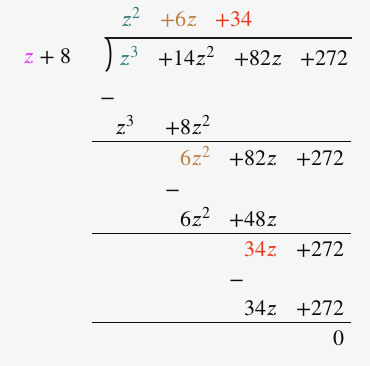
\includegraphics[scale=0.35]{lab3polynomial.png}
  \caption{Long division.}
\end{figure}

Then factor the result using your favourite method. 

$z^2+6z+34=z^2+2(z)(3) + 3^2 - 3^2 + 34=(z+3)^2-9+34=(z+3)^2+25=(z+3)^2+5^2=(z+3)^2-(5i)^2=(z+3-5i)(z+3+5i)$

\item Consider the polynomial
$$
p(z)=z^4+12 z^3+57 z^2+132 z+136
$$
Factor $p$ over the complex numbers, using the information that $\zeta_1=-2+2 i$ is a root of $p$.

\textbf{Solution:} Since coefficients for $p$ are all real numbers then the complex conjugate of $\zeta_1$ is also a root. Means $\zeta_2=-2-2i$. Then $(z-\zeta_1)(z-\zeta_2)=(z+2-2i)(z+2-2i)$. 

\begin{verbatim}
	>> syms z; simplify((z+2-2*i)*(z+2+2*i))
ans =
z^2 + 4*z + 8
\end{verbatim}

Perform corner division.

\begin{figure}[H]
\centering
  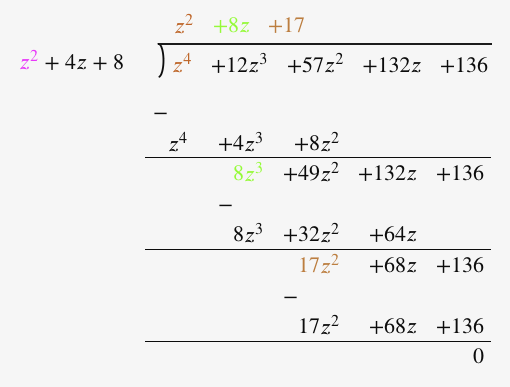
\includegraphics[scale=0.35]{lab3polynomialBIG.png}
  \caption{Long division.}
\end{figure}

Factor the result using your favourite method. $z^2+8z+17=z^2+2(z)(4) + 4^2 - 4^2 + 17 = (z+4)^2-16+17=(z+4)^2 + 1 = (z+4)^2 -(i)^2=(z+4-i)(z+4+i)$. Thus, we find $\zeta_3,\zeta_4.$

\item Dot product question is trivial. 

\textbf{Solution:} Use definition $u\cdot v = \| u \| \| v \| \cos(\widehat{uv})$, where $\| .\|$ is length. 

\item  An orthogonal set of vectors is a set of vectors in which every pair of vectors within the set are orthogonal to each other.
Among the sets of vectors listed below, identify the orthogonal ones. - Type ' 1 ' for 'orthogonal set', and type ' 0 ' for 'not orthogonal set'
$$
\begin{aligned}
& (-3,-3,-10,-40,-16),(10,-16,3,0,3),(33,-26,10,0,8) \\
& (21,53,-28,-20,1),(18,14,12,55,316),(0,-1300,-3195,1028,0) \\
& (-3,-10),(-10,3),(3,10) \\
& (53,12,1),(-40,26,1808),(21670,-95864,1858) \\
& (-8,1,-16),(12,320,14),(5134,-80,-2572),(-20,12,-8)
\end{aligned}
$$

\textbf{Solution:} Use dot product property - the dot product of perpendicular vectors means $\cos(\theta)=\cos(90^\circ)=0$, hence their dot product is zero. (Since it is online quiz you might want to use a calculator).

\end{enumerate}

\section{Lab 4}

\section{Lab 5}
\subsection{Practice problems}
\begin{enumerate}
	\item (a) Solve the following system of linear equations by first forming its augmented matrix and then row reducing it to reduced row echelon form. Give the answer in vector form. Show all of your steps and indicate the row operation performed at each step.
$$
\begin{array}{r}
x_1-3 x_2+2 x_3-x_4+2 x_5=2 \\
3 x_1-9 x_2+7 x_3-x_4+3 x_5=7 \\
2 x_1-6 x_2+7 x_3+4 x_4-5 x_5=7
\end{array}
$$

\textbf{Solution:}
$$
\begin{aligned}
& x_1-3 x_2+2 x_3-x_4+2 x_5=2 \\
& 3 x_1-9 x_2+7 x_3-x_4+3 x_5=7 \\
& 2 x_1-6 x_2+7 x_3+4 x_4-5 x_5=7
\end{aligned}
$$
lets form its augmented matrix and Row reduce it to RREF
$$
\left[\begin{array}{ccccc|c}
1 & -3 & 2 & -1 & 2 & 2 \\
3 & -9 & 7 & -1 & 3 & 7 \\
2 & -6 & 7 & 4 & -5 & 7
\end{array}\right] \underset{-2 R_1}{-3 R_1} \rightarrow\left[\begin{array}{ccccc|c}
1 & -3 & 2 & -1 & 2 & 2 \\
0 & 0 & 1 & 2 & -3 & 1 \\
0 & 0 & 3 & 6 & -9 & 3
\end{array}\right]-3 R_2
$$
solve for pivots
$\rightarrow\left[\begin{array}{ccccc|c}1 & -3 & 0 & -5 & 8 & 0 \\ 0 & 0 & 1 & 2 & -3 & 1 \\ 0 & 0 & 0 & 0 & 0 & 0\end{array}\right]$
$$
\begin{aligned}
& x_1-3 x_2-5 x_4+8 x_5=0, \\
& x_3+2 x_4-3 x_5=1, \\
& x_1=0+3 x_2+5 x_4-8 x_5, \\
& x_3=1-2 x_4+3 x_5,
\end{aligned}
$$
Then $x_2, x_4, x_5$ - free variables, let $x_2=s, x_4=t$,
$x_s=q$, for some si. $g \in R$, then:
and $A$ vector form:
$$
x=\left[\begin{array}{l}
0 \\
0 \\
1 \\
0 \\
0
\end{array}\right]+\left[\begin{array}{l}
3 \\
1 \\
0 \\
0 \\
0
\end{array}\right] S+\left[\begin{array}{c}
5 \\
0 \\
-2 \\
1 \\
0
\end{array}\right] t+\left[\begin{array}{c}
-8 \\
0 \\
3 \\
0 \\
1
\end{array}\right] g
$$
$x=\left[\begin{array}{l}0 \\ 0 \\ 1 \\ 0 \\ 0\end{array}\right]+\left[\begin{array}{l}3 \\ 1 \\ 0 \\ 0 \\ 0\end{array}\right] s+\left[\begin{array}{c}5 \\ 0 \\ -2 \\ 1 \\ 0\end{array}\right] t+\left[\begin{array}{c}-8 \\ 0 \\ 3 \\ 0 \\ 1\end{array}\right] g$, for some $s, t, g \in \mathbb{R}$.


(b) Find all vectors $\left[\begin{array}{l}a \\ b\end{array}\right] \in \mathbb{R}^2$ such that the solution to the linear system with augmented matrix
$$
\left[\begin{array}{ll|l}
1 & 2 & a \\
3 & 2 & b
\end{array}\right]
$$
is the vector $\left[\begin{array}{l}-a \\ -b\end{array}\right]$. Show your work.
\textbf{Solution:}
b) $\left[\begin{array}{ll|l}1 & 2 & a \\ 3 & 2 & b\end{array}\right]$ let's find RREF of this matrix
$$
\left[\begin{array}{ll|l}
1 & 2 & a \\
3 & 2 & b
\end{array}\right]_{-3 R_1} \rightarrow\left[\begin{array}{cc|c}
1 & 2 & a \\
0 & -4 & b-3 a
\end{array}\right]: \underset{(-4)}{\rightarrow}\left[\begin{array}{cc|c}
1 & 2 & a \\
0 & 1 & \frac{3 a-b}{4}
\end{array}\right]-2 R_2
$$
$=\left[\begin{array}{cc|c}1 & 0 & a-2\left(\frac{3 a-b}{y_2}\right) \\ 0 & 1 & \frac{3 a-b}{4}\end{array}\right] \rightarrow\left[\begin{array}{ll|l}1 & 0 & \frac{-a+b}{2} \\ 0 & 1 & \frac{3 a}{4}-\frac{b}{4}\end{array}\right]$, therefore $x_1=-\frac{a}{2}+\frac{b}{2}$ $x_2=\frac{3 a}{4}-\frac{b}{4}$ and from the assumption we know that the solution is $\left[\begin{array}{l}-a \\ -b\end{array}\right]$, $x_2=\frac{3 a}{4}-\frac{b}{4}$
then: $\begin{aligned} & -a=-\frac{a}{2}+\frac{b}{2} \\ & -b=\frac{3 a}{4}-\frac{b}{4}\end{aligned}$, lets solve for $a$ and $b$ :
$a-\frac{a}{2}=-\frac{b}{2} \rightarrow \frac{a}{2}+\frac{b}{2}=0$, lets form its matrix:
$b-\frac{b}{4}=-\frac{3 a}{4} \quad \frac{3 a}{4}+\frac{3 b}{4}=0$
$\left[\begin{array}{ll|l}\frac{1}{2} & \frac{1}{2} & 0 \\ \frac{3}{4} & \frac{3}{4} & 0\end{array}\right]$, lets Row Reduce it to the RREF:
$$
\left[\begin{array}{ll|l}
\frac{1}{2} & \frac{1}{2} & 0 \\
\frac{3}{4} & \frac{3}{4} & 0
\end{array}\right] \cdot 2 \rightarrow\left[\begin{array}{ll|l}
1 & 1 & 0 \\
3 & 3 & 0
\end{array}\right]-3 R_1 \rightarrow\left[\begin{array}{ll|l}
1 & 1 & 0 \\
0 & 0 & 0
\end{array}\right],
$$
Therefore, $b$ is a free variable, let $b=t$, for some $t \in R$.
$\quad\left[\begin{array}{l}a \\ b\end{array}\right]=\left[\begin{array}{c}-1 \\ 1\end{array}\right] t$, for some $t \in R$
\item Let $\mathbf{u}, \mathbf{v}, \mathbf{w}, \mathbf{x}, \mathbf{y} \in \mathbb{R}^n$.

(a) Prove the following statement:
If $\mathbf{u} \in \operatorname{Span}(\mathbf{w}+3 \mathbf{x}, \mathbf{x}+3 \mathbf{y})$, then $\mathbf{u} \in \operatorname{Span}(\mathbf{w}, \mathbf{x}, \mathbf{y})$.

(b) Give a counterexample using vectors in $\mathbb{R}^3$ to show that the following statement is false:
If $\mathbf{v} \in \operatorname{Span}(\mathbf{w}, \mathbf{x}, \mathbf{y})$, then $\mathbf{v} \in \operatorname{Span}(\mathbf{w}+3 \mathbf{x}, \mathbf{x}+3 \mathbf{y})$

\textbf{Solution is straightforward, use the definition of span.}
\item The augmented matrix $M$ below represents a system of linear equations, where $a \in \mathbb{R}$.
$$
M=\left[\begin{array}{ccc|c}
1 & 1 & 3 a+1 & 2-3 a \\
2 & a & 2 & -8 \\
-1 & -1 & a^2-2 a-3 & a^2
\end{array}\right]
$$
(a) Reduce the matrix $M$ to a row echelon form. Show your work.

(b) Find all $a \in \mathbb{R}$ so that the system has infinitely many solutions. Justify your answer.

(c) Find all $a \in \mathbb{R}$ so that the system has no solution. Justify your answer.

(d)  Find all $a \in \mathbb{R}$ so that the system has a unique solution. Justify your answer.

\textbf{Solution:}

(a) \begin{equation}
\begin{aligned}
& \text { a) }\left[\begin{array}{ccc|c}
1 & 1 & 3 a+1 & 2-3 a \\
2 & a & 2 & -8 \\
-1 & -1 & a^2-2 a-3 & a^2
\end{array}\right]\underset{+R_1}{-2 R_1} \rightarrow\left[\begin{array}{ccc|c}
1 & 1 & 3 a+1 & 2-3 a \\
0 & a-2 & -6 a & -8-2(2-3 a) \\
0 & 0 & a^2-2 a-3+3 a+1 & a^2+2-3 a
\end{array}\right] \\
& \rightarrow\left[\begin{array}{ccc|c}
1 & 1 & 3 a+1 & 2-3 a \\
0 & a-2 & -6 a & 6 a-12 \\
0 & 0 & (a-1)(a+2) & (a-2)(a-1)
\end{array}\right] \\
& \text { REF of mAtrix }(M): \quad\left[\begin{array}{ccc|c}
1 & 1 & 3 a+1 & 2-3 a \\
0 & a-2 & -6 a & 6 a-12 \\
0 & 0 & (a-1)(a+2) & (a-2)(a-1)
\end{array}\right] \text {. } \\
&
\end{aligned}
\end{equation}

(b) for system to have infinitely many solutions, we weed a free variable, which means a column without pivot.
Let $a=1$, then:
$$
\left[\begin{array}{ccc|c}
1 & 1 & 3+1 & 2-3 \\
0 & 1-2 & -6 & 6-12 \\
0 & 0 & (1-1)(1+2) & (1-2)(1-1)
\end{array}\right] \rightarrow\left[\begin{array}{ccc|c}
1 & 1 & 4 & -1 \\
0 & -1 & -6 & -6 \\
0 & 0 & 0 & 0
\end{array}\right]
$$
So, if $a=1$ there is a free variable. column without a pivot.
Let $a=2$, then
$$
\left[\begin{array}{ccc|c}
1 & 1 & 3 \cdot 2+1 & 2-3 \cdot 2 \\
0 & 2-2 & -6 \cdot 2 & 6 \cdot 2-12 \\
0 & 0 & (2-1)(2+2) & (2-2)(2-1)
\end{array}\right] \quad\left[\begin{array}{ccc|c}
1 & 1 & 7 & -4 \\
0 & 0 & -12 & 0 \\
0 & 0 & 4 & 0
\end{array}\right]
$$
So, if $a=2$ there is a free variable. column without pivot.

(c) System will have no solution if $\operatorname{Rank}(A)<\operatorname{Rank}(A \mid b)$. Let $a=-2$, then:
$$
\begin{aligned}
& {\left[\begin{array}{ccc|c}
1 & 1 & 3(-2)+1 & 2-3(-2) \\
0 & -2-2 & -6(-2) & 6(-2)-12 \\
0 & 0 & (-2-1)(-2+2) & (-2-2)(-2-1)
\end{array}\right] \quad\left[\begin{array}{ccc|c}
1 & 1 & -5 & 8 \\
0 & -4 & 12 & -24 \\
0 & 0 & 0 & 12
\end{array}\right]} \\
& {\left[\begin{array}{ccc|c}
1 & 1 & -5 & 8 \\
0 & -4 & 12 & -24 \\
0 & 0 & 0 & 12
\end{array}\right]=(A \mid b) \quad \operatorname{Rank}(A)=2, \operatorname{Rank}(A \mid b)=3,} \\
& \operatorname{Rank}(A)<\operatorname{Rank}(A \mid b)
\end{aligned}
$$
Therefore, if $a=-2$, then the system will be inconsistent.

(d) $\left[\begin{array}{ccc|c}1 & 1 & 3 a+1 & 2-3 a \\ 0 & a-2 & -6 a & 6 a-12\end{array}\right]$

The system will have only one solution if $a-2 \neq 0$ and $(a-1)(a+2) \neq 0$

$a-2=0$, if $a=2$.

$(a-1)(a+2)=0$, if $a=1, a=-2$.

Which means, that the system will have only one solution if 

$a \neq 1, a \neq-2, a \neq 2 \implies a \in(-\infty,-2) \cup(-2,1) \cup(1,2) \cup(2, \infty)$.

Therefore, the system has only one solution if $a \in(-\infty,-2) \cup(-2,1) \cup(1,2) \cup(2, \infty)$.

\end{enumerate}

\section{Lab 6}
When solving matrix equation it is better to first express unknown in terms of known matrices and then substitute the values in. 
\begin{align*}
\left(A^T C-X\right)^T=C A+A C\\
A^T C - X=\left(CA + AC\right))^T\\
X = A^T C - \left(CA + AC\right))^T
\end{align*}

Symmetric, skew symmetric proofs. 
To prove that the matrix is symmetric the most straightforward way is to prove that two elements mirrored against the main diagonal $a_{ij}=a_{ji}$  are equal (for skew symmetric $a_{ij}=-a_{ji}$).
However, this might involve heavy computations. Need to prove that $(A)^T=A$. We can always make it easier. 

\textbf{Example 1}: Let $A$ be an $n\times n$ symmetric matrix. Show that $2 A^2-28A+I$ is symmetric. 

\textit{Note: $I$ is an identity matrix with 1 on main diagonal and 0 everywhere else.}

\textbf{Proof:}

Consider $A^2$, we have $(A^2)^T=(AA)^T=A^TA^T=($since $A$ is symmetric $)=AA=A^2$. Here we used the property that $(LK)^T=K^TL^T$.

Now $2A^2$ and $28A$ are also symmetric, since multiplying the whole matrix by a scalar makes each element of the matrix multiplied by that scalar ($ba_{ij}=ba_{ji},b\in \mathbb{R},a_{ij}\in A$). 

Last step. $(2A^2-28A+I)^T=(2A^2)^T-(28A)^T+I^T=2A^2-28A+I$ where we used symmetricity of $2A^T$, $28A$ and $I$. Q.E.D.

\textbf{Example 2:} Prove that $A B A^T$ is symmetric when $B$ is symmetric matrix.

\textbf{Proof:} $$\left(A B A^T\right)^T=\left((A B) A^T\right)^T=(A^T)^T(A B)^T=\left(A^T\right)^T(B)^T(A)^T=A B^T A^T.$$

Since $B$ is symmetric, then $B^T=B$. Which means the equation continues as $A B A^T$. Q.E.D

\textbf{Example 3:} For any square matrix $A$, prove that $\frac{1}{2}\left(A+A^T\right)$ is symmetric.

\textbf{Proof:}

The property is easy to prove if you know that:
\begin{itemize}
\item[(1)]	$\left(A^T\right)^T=A$
\item[(2)]   $(A+B)^T=A^T+B^T$
\end{itemize}

Use this on $X=\frac{1}{2}\left(A+A^T\right)$ to find that $X^T=X$, and thus $X$ is symmetric.
$$
X^T=\frac{1}{2}\left(A+A^T\right)^T=\frac{1}{2}\left(A^T+\left(A^T\right)^T\right)=\frac{1}{2}\left(A^T+A\right)=\frac{1}{2}\left(A+A^T\right)=X.
$$

\textbf{Example 4:}

Is $\left(A^{-1}\right)^T=\left(A^T\right)^{-1}$?.

\textbf{Proof:}

Use the definition of invertibility. Given $M$ if there is $N$ such that $MN=I$ and $NM=I$ we say that $\mathrm{A}$ is invertible and we call $N=M^{-1}$.

$$
\begin{aligned}
& A^T\left(A^{-1}\right)^T=\left(A^{-1} A\right)^T=I^T=I \\
& \left(A^{-1}\right)^T A^T=\left(A A^{-1}\right)^T=I^T=I
\end{aligned}
$$
This proves that the inverse of $A^T$ is $\left(A^{-1}\right)^T$. 

\newpage\textbf{Example 5:} Prove or disprove that square invertible matrices form a group under matrix multiplication. 

\textbf{Proof:}

If invertible matrices with real entries form a group, we need to check each of the group requirements:
\begin{itemize}
\item[(1)] \textit{Closed under operation:} Multiplication of matrices in our set produces matrices of the same set. Let $A, B$ be invertible $n\times n$. Then $A B$ is certainly a $n \times n$ matrix, and $A B$ is invertible, as $(A B)^{-1}=B^{-1} A^{-1}$, and by definition of group of square invertible matrices $B^{-1}$ and $A^{-1}$ exist and are elements of the group.
\item[(2)] \textit{Associativity: }The group operation is associative, as matrix multiplication is associative.
\item[(3)] \textit{Identity element: }The identity is $I$, so an identity element exists and is part of the group.
\item[(4)] \textit{Invertibility:} Every element of the set has an inverse by definition.
\end{itemize}

All entries are satisfied, hence it is a group. Q.E.D.

\section{Eigenvalues and eigenvectors}

Consider the plane $W$ in $\mathbb{R}^3$ through the origin $2x+2y-z=0$. Let $P:\mathbb{R}^3\to\mathbb{R}^3$ denote \textbf{orthogonal projection} of $\mathbb{R}^3$ onto $W$ and let $R:\mathbb{R}^3\to\mathbb{R}^3$ denote the \textbf{reflection} of $\mathbb{R}^3$ about $W$. 

Let $\vec{x}\in\mathbb{R}^3$ be eigenvector, $\lambda_i\in \mathbb{R}$ eigenvalues, then the projection:
\begin{equation}\label{proj}
	P\vec{x}=\vec{x}_{\operatorname{proj}},\text{ and }P\vec{x}=\lambda\vec{x}.
\end{equation}
If we apply projection twice, the resulting vector does not change:
\begin{equation}\label{doubleproj}
	P^2\vec{x}=\vec{x}_{\operatorname{proj}},\text{ and }P^2\vec{x}=\lambda^2\vec{x}	.
\end{equation}

Combining equations~\eqref{proj}-\eqref{doubleproj} lead to:
\begin{equation*}
	\vec{x}_{\operatorname{proj}}=\vec{x}_{\operatorname{proj}}\iff\lambda \vec{x}=\lambda^2\vec{x}\iff \left(\lambda^2-\lambda\right)\vec{x}=0\iff \lambda=0,1. \text{ Trivial solution }\vec{x}=\vec{0}.
\end{equation*}
These are the only possible eigenvalues for the projection operator. 

Next, consider vector $\vec{w}$ belonging to the plane $\vec{w}\in W\implies$
\begin{equation*}
	\exists \{\vec{x}_1,\vec{x}_2\}\subset W \text{ lin.indep.}, \{\alpha,\beta\}\subset \mathbb{R}:\vec{w}=\alpha\vec{x}_1+\beta\vec{x}_2\text{ and }P(\vec{w})=\lambda\vec{w}=\lambda\left(\alpha\vec{x}_1+\beta\vec{x}_2\right)=\alpha\vec{x}_1+\beta\vec{x}_2=\vec{w}\text{, where }\lambda=1.
\end{equation*}
We may also consider vector $\vec{n}$ in $W^\perp$, which is normal to the plane $W$, $\vec{n}\in W^\perp\implies$
\begin{equation*}
	\exists \vec{x}_3\in W^\perp, \gamma \in \mathbb{R}:\vec{n}=\gamma \vec{x}_3\text{ and }P(\vec{n})=\lambda\vec{n}=\lambda\gamma \vec{x}_3=0\gamma \vec{x}_3=0\text{, where }\lambda=0.	
\end{equation*}

The above procedure can be repeated for the reflection operator $R$, with one exception that few algebraic steps are needed. Subtracting two projections is equivalent to the reflection, which reads as
\begin{align*}
	R 	&=I-2P,\text{ then we consider double reflection}\\
	R^2 &=(I-2P)(I-2P)\\
		&=I^2-I2P-2PI+2P2P\\
		&=I-2IP-2PI+4P^2\\
		&=I-2P-2P+4P^2\\
		&=I-4P+4P^2\\
		&=I-4P+4P\\
		&=I,
\end{align*}
which is, indeed, true, because reflecting the vector twice maps it to itself. Hence,
\begin{equation*}
	R^2\vec{x}=\lambda^2{x},\text{ on the other hand } R^2\vec{x}=I\vec{x}=\vec{x},
\end{equation*}
therefore
\begin{equation*}
	\lambda^2{x}=\vec{x}\iff\left(\lambda^2-1\right)\vec{x}=0\iff\lambda=\pm1.\text{ Trivial solution }\vec{x}=\vec{0}.
\end{equation*}

Now, we represent both $\vec{w},\vec{n}$ the same as in the projection part. If $\vec{w}$ lies on plane $W$, then it can be represented as a linear combination of linearly independent eigenvectors $\vec{x}_1,\vec{x}_2$ which form a basis on plane $W$. Similarly, $\vec{n}$ can be represented as a scaled version of an eigenvector $\vec{x}_3$, which spans $W^\perp$. Writing down:
\begin{align*}
	\vec{w}&=\alpha\vec{x}_1+\beta\vec{x}_2,\{\alpha,\beta\}\subset \mathbb{R},\\
	\vec{n}&=\gamma\vec{x}_3,\gamma\in\mathbb{R}.
\end{align*}
Then, after applying reflection to $\vec{w},\vec{n}$ we get:
\begin{align*}
	R(\vec{w})&=\lambda\vec{w}=\lambda\left(\alpha\vec{x}_1+\beta\vec{x}_2\right)=\alpha\vec{x}_1+\beta\vec{x}_2=\vec{w},\lambda=1,\\
	R(\vec{n})&=\lambda\vec{n}=\lambda\gamma\vec{x}_3=-\gamma\vec{x}_3=-\vec{n},\lambda=-1.
\end{align*}



\bibliographystyle{plain}
\bibliography{Zotero}

\appendix

\section{Appendix}


\end{document}

